Now that the position of graphene for every point in the $x,y$-plane is known the electric field can be projected onto this plane. This projection yields another slice, now in the plane of graphene:

\begin{minted}{matlab}
  x_length = length(obj.x);
  y_length = length(obj.y);
  grid_size= 0.5;
  data = ones(x_length, y_length);
  for x_loop=1:x_length
     for y_loop=1:y_length
         height = map.height(x_loop, y_loop);
         [~, index] = min(abs(obj.z - height));
         sliceX = obj.Ex(x_loop,y_loop,index);
         sliceY = obj.Ey(x_loop,y_loop,index);
         sliceZ = obj.Ey(x_loop,y_loop,index);
         height_next_x = map.height(x_loop+1, y_loop);
         height_next_y = map.height(x_loop+1, y_loop);
         x_projection = cos(atan((height_next_x - height) / grid_size));
         y_projection = cos(atan((height_next_y - height) / grid_size));
         z_projection = 1 - cos(atan((height_next_y - height) / grid_size));
         data(x_loop, y_loop) = sliceX .* conj(sliceX) * x_projection +
            sliceY .* conj(sliceY) * y_projection +
            sliceZ .* conj(sliceZ) * z_projection;
     end
  end
  graphene_slice = slice(data, obj.x, obj.y);
\end{minted}

The returned slice now is just a regular slice which can be plotted as seen in figure \ref{fig:projected}.

\begin{figure}[!h]
  \centering
  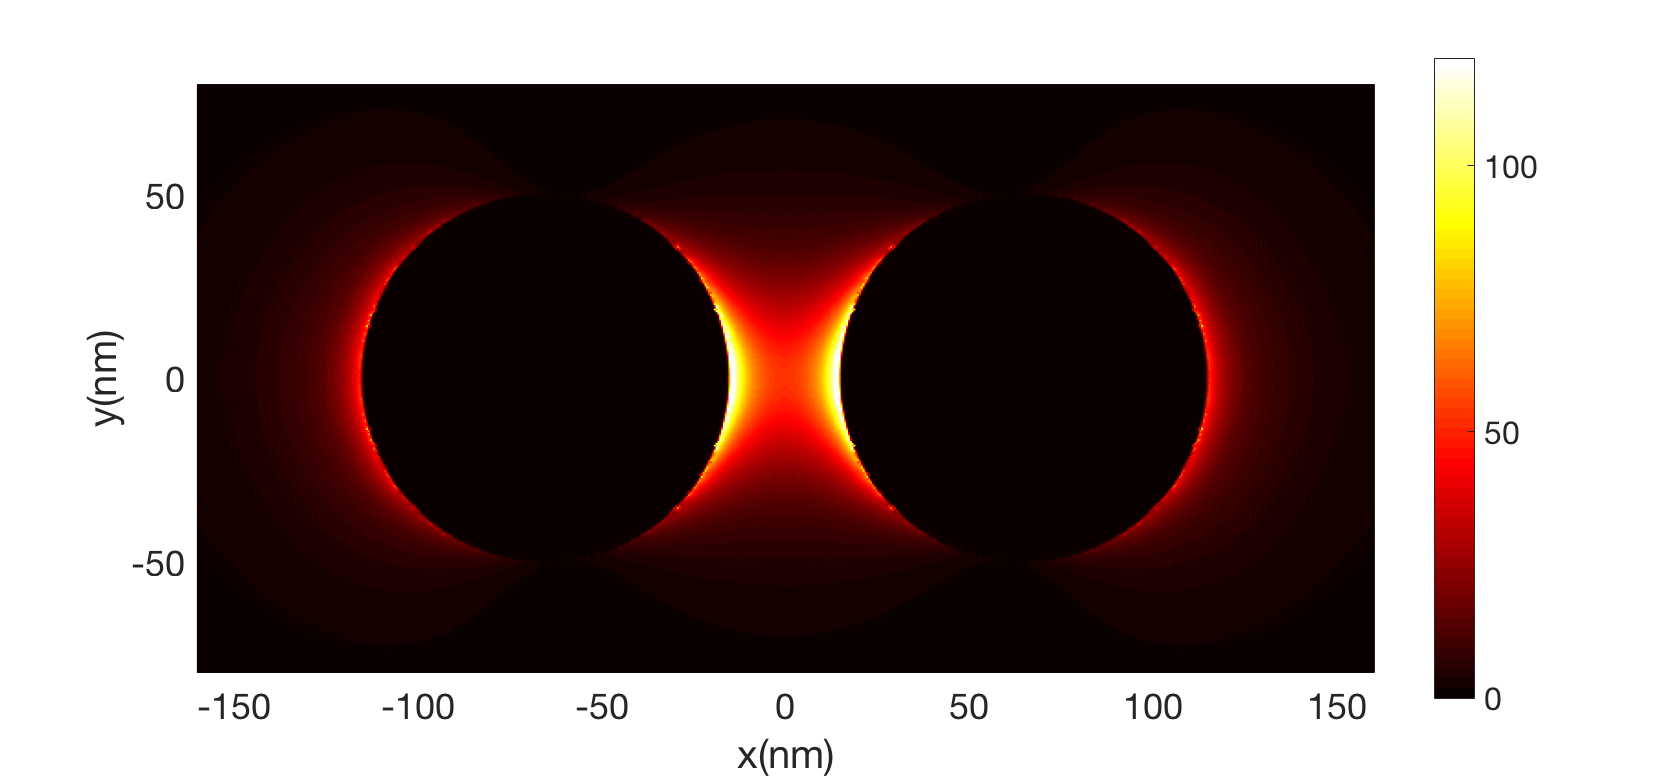
\includegraphics[width=\textwidth]{./images/graphene-layer.png}
  \caption{Near field enhancement $|E/E_0|^2$ in the layer of graphene after applying the height map.}
  \label{fig:projected}
\end{figure}
